\chapter{Krei movadon}
{ }\hfill\textbf{Nivelo:} meza

^Ci tiu ^capitro proponas du aferojn tre malsamajn kies celo estas krei
movadon per \xlogo.

\section{La ciferoj de la kalkulilo}

\begin{center}
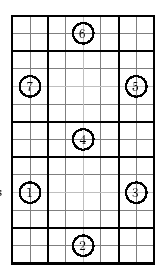
\includegraphics{bildoj/animation-chiffre.png}
\end{center}

^Ci tiu tasko bazi^gas sur la fakto ke ^ciun kalkulilan nombron oni
povas akiri per la jena ^sablono:
\begin{itemize}
\item Por ekzemplo, por desegni \og 4\fg, oni ^saltu l' ortangulojn 3, 4, 5, 7.
\item Por desegni \og 8\fg, oni ^saltu l' ortangulojn 1, 2, 3, 4, 5, 6, 7.
\item Por desegni \og 3\fg, oni ^saltu l' ortangulojn 2, 3, 4, 5, 6.
\end{itemize}

\subsection{Plenigi ortangulon}
\begin{center}
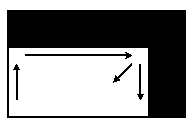
\includegraphics{bildoj/animation-rectangle.png}
\end{center}
Se oni deziras ekzemple grafiki plenan ortangulon grandan je $100$ mul
$200$, unua ideo povas esti desegni la ortangulon je $100$ mul $200$,
poste desegni ortangulon je $99$ mul $199$, poste ortangulon je $98$
mul $198$... ^gis la ortangul' estos tute plena.

Ni komencu per difini ortangulon je lango kaj lar^go dependaj je du
variabloj.
\begin{verbatim}
por ort :lo :la
ripetu 2 [an :lo dn 90 an :la dn 90]
fino
\end{verbatim}
Por plenigi nian grandan ortangulon, oni rulu:

\texttt{ort 100 200 ort 99 199 ort 98 198  ..... ort 1 101}

Difinu tiam proceduron ortangulo dedi^cita grafiki tiun plenan ortangulon.
\begin{verbatim}
por ortangulo :lo :la
ort :lo :la
ortangulo :lo-1 :la-1
fino
\end{verbatim}
Oni provu \texttt{ortangulo 100 200} kaj oni rimarku ke estas
problemo: la proceduro ne haltas kiam la ortangulo estas plena; ^gi
plu grafikas ortangulojn!  Oni do aldonu provon ebligantan detekti ^cu
la longo a^u la lar^go egalas $0$.  Tiam, oni petas la programon halti
per la komando \texttt{haltu}.
\begin{verbatim}
por ortangulo :lo :la
se aŭ :lo=0 :la=0 [haltu]
ort :lo :la
ortangulo :lo-1 :la-1
fino
\end{verbatim}
Rimarko: anstata^u uzi la primitivon \texttt{a^u}, oni povas uzi la
simbolon \og|\fg; oni skribus:
\begin{center}
\texttt{se :lo=0 | :la=0 [haltu]}
\end{center}

\subsection{La programo}
\noindent Ni bezonas la plenan ortangulon anta^uan:
\begin{verbatim}
por ort :lo :la
se :lo=0 |:la=0 [haltu]
ripetu 2 [an :lo dn 90 an :la dn 90]
ort :lo-1 :la-1
fino
\end{verbatim}

Ni supozas ke la testudo ekiras de la malsupra maldekstra angulo.  Ni
difinos proceduron nomatan \texttt{cifero} akceptantan $7$ argumentojn
\texttt{:a}, \texttt{:b}, \texttt{:c}, \texttt{:d}, \texttt{:e},
\texttt{:f}, \texttt{:g}.  Kiam \texttt{:a} valoras $1$, oni desegnu
la ortangulon $1$.  Se \texttt{:a} valoras $0$, oni ne desegnu ^gin.
Jen la principo.

Jen la proceduro:
\begin{verbatim}
por cifero :a :b :c :d :e :f :g
# Oni desegnu la ortangulon 1
se :a=1 [ort 160 40]
# Oni desegnu la ortangulon 2
se :b=1 [ort 40 160]
l dn 90 an 120 mdn 90 ml
# Oni desegnu la ortangulon 3
se :c=1 [ort 160 40]
l an 120 ml
# Oni desegnu la ortangulon 5
se :e=1 [ort 160 40]
# Oni desegnu la ortangulon 4
mdn 90 l man 40 ml
se :d=1 [ort 160 40]
# Oni desegnu la ortangulon 6
dn 90 l an 120 mdn 90 ml
se :f=1 [ort 160 40]
# Oni desegnu la ortangulon 7
l an 120 mdn 90 man 40 ml
se :g=1 [ort 160 40]
fino
\end{verbatim}
\subsection{Krei malgradan animadon}
^Ci tie ni simulos retronombradon aperigante sekvence la ciferojn de
$9$ ^gis $0$ je ordo malkreska.
\begin{verbatim}
por retronombro
ev tdk cifero 0 1 1 1 1 1 1 atendu 60
ev tdk cifero 1 1 1 1 1 1 1 atendu 60
ev tdk cifero 0 0 1 0 1 1 0 atendu 60
ev tdk cifero 1 1 1 1 0 1 1 atendu 60
ev tdk cifero 0 1 1 1 0 1 1 atendu 60
ev tdk cifero 0 0 1 1 1 0 1 atendu 60
ev tdk cifero 0 1 1 1 1 1 0 atendu 60
ev tdk cifero 1 1 0 1 1 1 0 atendu 60
ev tdk cifero 0 0 1 0 1 0 0 atendu 60
ev tdk cifero 1 1 1 0 1 1 1 atendu 60
fino
\end{verbatim}

Jen malgranda problemo: estas palpebruma efiko malagraba dum krei
^ciun ciferon.  Por fluemigi tion oni uzos la primitivojn
\texttt{movado}, \texttt{neplu\_movigu} kaj \texttt{novigu}.
\begin{itemize}
\item \texttt{movado} ebligas ^salti la moduson \og movado\fg.  La
  testudo ne desegnos plu sur l' ekrano, sed en bufro, tio estas, en
  memoro.  ^Gi aldonos la bildon nur kiam oni petos per la primitivo
  \texttt{novigu}.
\item \texttt{neplu\_movigu} ebligas mal^salti tiun moduson kaj reveni
  en la klasikan moduson.
\end{itemize}
Jen la modifita programo:
\begin{verbatim}
por retronombro
# Pasu en moduson movado
movado
ev tdk cifero 0 1 1 1 1 1 1 novigu atendu 60
ev tdk cifero 1 1 1 1 1 1 1 novigu atendu 60
ev tdk cifero 0 0 1 0 1 1 0 novigu atendu 60
ev tdk cifero 1 1 1 1 0 1 1 novigu atendu 60
ev tdk cifero 0 1 1 1 0 1 1 novigu atendu 60
ev tdk cifero 0 0 1 1 1 0 1 novigu atendu 60
ev tdk cifero 0 1 1 1 1 1 0 novigu atendu 60
ev tdk cifero 1 1 0 1 1 1 0 novigu atendu 60
ev tdk cifero 0 0 1 0 1 0 0 novigu atendu 60
ev tdk cifero 1 1 1 0 1 1 1 novigu atendu 60
# Revenu en moduson klasikan
neplu_movigu
fino
\end{verbatim}

\section{Animado: la hometo kiu kreskas}
\begin{center}
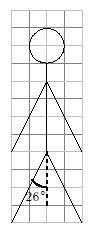
\includegraphics{bildoj/animation-bonhomme.png}
\end{center}
Anta^u ^cio, ni difinu proceduron \texttt{hometo} kiu grafikas la
hometon apudan je elektita amplekso.
\begin{verbatim}
por hometo :c
mdn 154 an 44*:c man 44*:c 
mdn  52 an 44*:c man 44*:c 
mdn 154 an 40*:c
mdn 154 an 44*:c man :c*44 
mdn  52 an 44*:c man :c*44 
mdn 154 an 10*:c
mdn  90 ripetu 180 [an :c/2 dn 2] dn 90
fino
\end{verbatim}
Nun ni kreos animadon ^sajnigantan ke la hometon kreskas po malmulte.
Por tio, ni grafikos \texttt{hometo 0.1}, poste \texttt{hometo 0.2},
\texttt{hometo 0.3}... ^gis \texttt{hometo 5}.  Inter ^ciu grafikado,
oni forvi^sos l' ekranon.  Jen la du proceduroj:
\begin{verbatim}
por hometo :c
mdn 154 an 44*:c man 44*:c 
mdn  52 an 44*:c man 44*:c 
mdn 154 an 40*:c
mdn 154 an 44*:c man :c*44 
mdn  52 an 44*:c man :c*44 
mdn 154 an 10*:c
mdn  90 ripetu 180 [an :c/2 dn 2] dn 90
se :c=5 [haltu]
ev tdk hometon :c+0.1
fino

por komenci
ev tdk
hometo 0
fino
\end{verbatim}
Finfine, por fluemigi la tuton, oni helpu sin per la moduson movado kaj la primitivo \texttt{novigu}.
\begin{verbatim}
por hometo :c
mdn 154 an 44*:c man 44*:c 
mdn  52 an 44*:c man 44*:c 
mdn 154 an 40*:c
mdn 154 an 44*:c man :c*44 
mdn  52 an 44*:c man :c*44 
mdn 154 an 10*:c
mdn  90 ripetu 180 [an :c/2 dn 2] dn 90
novigu
se :c=5 [haltu]
ev tdk hometo :c+0.1
fino

por komenci
tdk movado
hometo 0
neplu_movigu
fino

\end{verbatim}
\textbf{Rimarku: } Tie, la proceduro \texttt{hometo} estas rekurziva;
oni pli simple povus uzi la primitivon \texttt{ripetupor} por variigi
\texttt{:c} de $0.1$ ^gis $5$.  Jen la programo tiel:
\begin{verbatim}
por hometo :c
ev tdk mdn 154 an 44*:c man 44*:c 
mdn  52 an 44*:c man 44*:c 
mdn 154 an 40*:c
mdn 154 an 44*:c man :c*44 
mdn  52 an 44*:c man :c*44 
mdn 154 an 10*:c
mdn  90 ripetu 180 [an :c/2 dn 2] dn 90
novigu
fino

por komenci
tdk movado
ripetupor [c 0 5 0.1] [hometo :c]
neplu_movigu
fino

\end{verbatim}

